\documentclass{beamer}
\mode<presentation>
\usepackage{amsmath}
\usepackage{amssymb}
%\usepackage{advdate}
\usepackage{adjustbox}
\usepackage{subcaption}
\usepackage{enumitem}
\usepackage{multicol}
\usepackage{mathtools}
\usepackage{listings}
\usepackage{url}
\def\UrlBreaks{\do\/\do-}
\usetheme{Boadilla}
\usecolortheme{lily}
\setbeamertemplate{footline}
{
  \leavevmode%
  \hbox{%
  \begin{beamercolorbox}[wd=\paperwidth,ht=2.25ex,dp=1ex,right]{author in head/foot}%
    \insertframenumber{} / \inserttotalframenumber\hspace*{2ex} 
  \end{beamercolorbox}}%
  \vskip0pt%
}
\setbeamertemplate{navigation symbols}{}

\providecommand{\nCr}[2]{\,^{#1}C_{#2}} % nCr
\providecommand{\nPr}[2]{\,^{#1}P_{#2}} % nPr
\providecommand{\mbf}{\mathbf}
\providecommand{\pr}[1]{\ensuremath{\Pr\left(#1\right)}}
\providecommand{\qfunc}[1]{\ensuremath{Q\left(#1\right)}}
\providecommand{\sbrak}[1]{\ensuremath{{}\left[#1\right]}}
\providecommand{\lsbrak}[1]{\ensuremath{{}\left[#1\right.}}
\providecommand{\rsbrak}[1]{\ensuremath{{}\left.#1\right]}}
\providecommand{\brak}[1]{\ensuremath{\left(#1\right)}}
\providecommand{\lbrak}[1]{\ensuremath{\left(#1\right.}}
\providecommand{\rbrak}[1]{\ensuremath{\left.#1\right)}}
\providecommand{\cbrak}[1]{\ensuremath{\left\{#1\right\}}}
\providecommand{\lcbrak}[1]{\ensuremath{\left\{#1\right.}}
\providecommand{\rcbrak}[1]{\ensuremath{\left.#1\right\}}}
\theoremstyle{remark}
\newtheorem{rem}{Remark}
\newcommand{\sgn}{\mathop{\mathrm{sgn}}}
\providecommand{\abs}[1]{\left\vert#1\right\vert}
\providecommand{\res}[1]{\Res\displaylimits_{#1}} 
\providecommand{\norm}[1]{\lVert#1\rVert}
\providecommand{\mtx}[1]{\mathbf{#1}}
\providecommand{\mean}[1]{E\left[ #1 \right]}
\providecommand{\fourier}{\overset{\mathcal{F}}{ \rightleftharpoons}}
%\providecommand{\hilbert}{\overset{\mathcal{H}}{ \rightleftharpoons}}
\providecommand{\system}{\overset{\mathcal{H}}{ \longleftrightarrow}}
	%\newcommand{\solution}[2]{\textbf{Solution:}{#1}}
%\newcommand{\solution}{\noindent \textbf{Solution: }}
\providecommand{\dec}[2]{\ensuremath{\overset{#1}{\underset{#2}{\gtrless}}}}
\newcommand{\myvec}[1]{\ensuremath{\begin{pmatrix}#1\end{pmatrix}}}
\let\vec\mathbf

\lstset{
    basicstyle=\ttfamily,
    frame=single,
    breaklines=true,
    columns=fullflexible,
}
\numberwithin{equation}{section}
\title{Matgeo Presentation}
\author{Pushkar Gudla \\ AI24BTECH11012\\IIT Hyderabad.}
\date{\today} 

\begin{document}

\begin{frame}
\titlepage
\end{frame}

\section*{Outline}
\begin{frame}{Contents}
\tableofcontents    
\end{frame}

\section{Problem}
\begin{frame}{Problem Statement}
    The area of the region bounded by the curve $x^2=4y$ and the straight line $x=4y-2$ is
\end{frame}

\section{Solution}
\subsection{Setup and Variable Definitions}
\begin{frame}{Setup and Variable Definitions}
\begin{table}[h!]    
  \centering
  \begin{tabular}[15pt]{ |c| c|}
    \hline
    \textbf{Variable} & \textbf{Description}\\ 
    \hline
    $a$ & Length of side $BC$ \\
    \hline 
    $b$ & Length of side $AC$ \\
	\hline
    $c$ & Length of side $AB$ \\
    \hline
	$k$ & $k=b-c$ \\
	\hline
    \end{tabular}

  \caption{Variables and given data}
\end{table}
\end{frame}

\subsection{Converting to Matrix form}
\begin{frame}{Converting the equations to Matrix form}
    To simplify the calculation of points of intersection, the curve $x^2=4y$ is represented in standard conic matrix form:
    \begin{align}
        g(x) &= x^\top \vec{V}x + 2\vec{u}^\top x + f=0\\
        \vec{V} &= \myvec{1 & 0\\0 & 0}\\
	\vec{u} &= \myvec{0\\2}\\
	f &= 0
    \end{align}
\end{frame}

\subsection{Parametric Form of the Line}
\begin{frame}{Parametric Form of the Line}
	\begin{align}
	L: \vec{x} &= \vec{h}+k\vec{m} 
 \end{align}
 where $k$ is a scalar constant\\
 \begin{align}
        \vec{h} &= \myvec{-2 \\ 0}\\
	\vec{m} &= \myvec{1 \\ \frac{1}{4}}\\
	\vec{x_i} &= \vec{h}+k_{i}\vec{m}
 \end{align}
\end{frame}

\subsection{Finding Points of Intersection}
\begin{frame}{Finding Points of Intersection}
On substituting $L$ in $g(x)$ we get a quadratic equation in $k$. We find that the discriminant is not equal to zero and thus we get two values $k_1$ and $k_2$.
The point obtained by substituting $k_1$ in $L$ is $\vec{x_1}$ and similarly on substituting $k_2$ in $L$ we get $\vec{x_2}$.
\begin{align}
	k_1 &= \frac{1}{\vec{m}^\top \vec{V}\vec{m}}\brak{-m^\top\brak{\vec{V}\vec{h}+\vec{u}}+ \sqrt{[\vec{m}^\top \brak{\vec{V}\vec{h}+\vec{u}}]^2 - g(\vec{h})\brak{\vec{m}^\top\vec{V}\vec{m}}}} \\
	k_2 &= \frac{1}{\vec{m}^\top \vec{V}\vec{m}}\brak{-m^\top\brak{\vec{V}\vec{h}+\vec{u}}- \sqrt{[\vec{m}^\top \brak{\vec{V}\vec{h}+\vec{u}}]^2 - g(\vec{h})\brak{\vec{m}^\top\vec{V}\vec{m}}}}
\end{align}
On solving for $k_1$ and $k_2$ we get $k_1=4$ and $k_2=1$. Thus
\begin{align}
    \vec{x_1} &= \myvec{2\\1}\\
    \vec{x_2} &= \myvec{-1\\ \frac{1}{4}}
\end{align}
\end{frame}

\subsection{Finding Area through Integration}
\begin{frame}{Finding Area through Integration}
    The area between the curve and the line from $x=-1$ to $x=2$ is calculated using the following integration:\\
    Area = $\int_{-1}^{2}\brak{\frac{x}{4}+\frac{1}{2}-\frac{x^2}{4}}dx$\\
    Solving this integral, we get Area=$\frac{9}{8}$.\\
    Hence, the area bound between the curve $x^2=4y$ and the line $x=4y-2$ is $\frac{9}{8}$.
\end{frame}

\section{Codes}
\subsection{C code to verify the Area}
\begin{frame}{C code to verify the Area}
We can use the following C code to verify that the area we found is correct.

\resizebox{\textwidth}{!}{\fbox{\url{https://github.com/GPushkar16/EE1030/blob/main/Matgeo/question-4/codes/area_between_curves.c}}}

\end{frame}

\subsection{Generating Parabola and Plotting the Figure}
\begin{frame}{Generating Parabola and Plotting the Figure}
    We can use the following C code to generate points that lie on the parabola:

    \resizebox{\textwidth}{!}{\fbox{\url{https://github.com/GPushkar16/EE1030/blob/main/Matgeo/question-4/codes/generate_parabola.c}}}


    We can then use the following Python code to generate the figure:
\resizebox{\textwidth}{!}{\fbox{\url{https://github.com/GPushkar16/EE1030/blob/main/Matgeo/question-4/codes/plot.py}}}

\end{frame}

\section{Figure}
\begin{frame}{Figure}
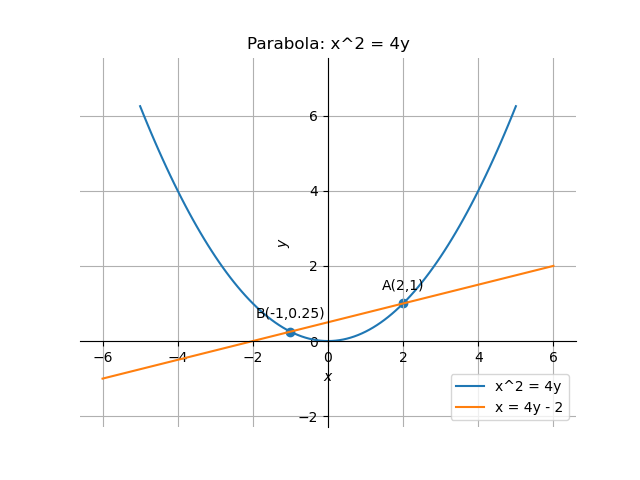
\includegraphics[width=0.8\textwidth]{figs/plot.png}
\end{frame}

\end{document}

